% This file was converted to LaTeX by Writer2LaTeX ver. 1.2
% see http://writer2latex.sourceforge.net for more info
\documentclass[twocolumn,a4paper]{article}
\usepackage[latin1]{inputenc}
\usepackage[T1]{fontenc}
\usepackage[english]{babel}
\usepackage{amsmath}
\usepackage{amssymb,amsfonts,textcomp}
\usepackage{color}
\usepackage{array}
\usepackage{hhline}
\usepackage{hyperref}
\hypersetup{dvips, colorlinks=true, linkcolor=blue, citecolor=blue, filecolor=blue, urlcolor=blue}
\usepackage[dvips]{graphicx}
% Outline numbering
\setcounter{secnumdepth}{0}
% Page layout (geometry)
\setlength\voffset{-1in}
\setlength\hoffset{-1in}
\setlength\topmargin{0.7874in}
\setlength\oddsidemargin{0.7874in}
\setlength\textheight{10.118099in}
\setlength\textwidth{6.6932993in}
\setlength\footskip{0.0cm}
\setlength\headheight{0cm}
\setlength\headsep{0cm}
% Footnote rule
\setlength{\skip\footins}{0.0469in}
\renewcommand\footnoterule{\vspace*{-0.0071in}\setlength\leftskip{0pt}\setlength\rightskip{0pt plus 1fil}\noindent\textcolor{black}{\rule{0.25\columnwidth}{0.0071in}}\vspace*{0.0398in}}
% Pages styles
\makeatletter
\newcommand\ps@Standard{
  \renewcommand\@oddhead{}
  \renewcommand\@evenhead{}
  \renewcommand\@oddfoot{}
  \renewcommand\@evenfoot{}
  \renewcommand\thepage{\arabic{page}}
}
\newcommand\ps@FirstPage{
  \renewcommand\@oddhead{}
  \renewcommand\@evenhead{}
  \renewcommand\@oddfoot{}
  \renewcommand\@evenfoot{}
  \renewcommand\thepage{\arabic{page}}
}
\makeatother
\pagestyle{Standard}
\title{}
\begin{document}
\clearpage\setcounter{page}{1}\pagestyle{Standard}
\thispagestyle{FirstPage}
\section{Cryptography \& Anonymity: }
\section{Ethical and Legal conflicts}
\clearpage
\bigskip

{\centering
Victor Rudolfsson
\par}

{\centering
H�gskolen i Gj�vik
\par}

{\centering
Gj�vik, Norge
\par}


\bigskip


\bigskip

In today's society, a growing number of organizations and governments advocate a centralized approach to safeguarding its own and its people's data, by introducing and enforcing laws\textsuperscript{[10]} and policies supposed to aid law enforcement. 

At the same time, a growing number of people and collectives sometimes referred to as ``\textit{cypherpunks}{}'' or ``\textit{cryptoanarchists''} advocate a decentralized solution to the safekeeping of data (and privacy) based on cryptographic algorithms.


\bigskip

A question we must ask ourselves is whether our data is ever safe, and who we wish to be responsible for keeping it safe. But more importantly, whether or not a centralized approach is useful to begin with. Many of these laws meant to harvest, store and index data are said to be meant for enforcing other laws, such as stopping the distribution of child pornography, finding and arresting terrorists, and stopping financial fraud. 


\bigskip

However, when a majority of a country's population is monitored most of, or all the time, and their communications stored and indexed, can this information really be used to aid law enforcement when those who these laws are meant to stop can easily avoid them by utilizing transfer protocols based on cryptographic algorithms to secure communication end-to-end? And do such protocols actually pose a problem for law enforcement?


\bigskip

There are many different techniques to encrypt data transmission, and there are several alternatives providing different kinds of security as well (\textit{IPSec}, \textit{SSL} \& \textit{PPTP} for VPN, \textit{SSL }or \textit{SSL/TLS}, TOR\textsuperscript{[4]} or I2P and so on), but this paper will try to briefly explain how a few of the most commonly used encryption protocols for data communication work, and find out whether or not communication can be safeguarded in a decentralized manner, if a centralized approach is required and if these two approaches conflict with each other.


\bigskip

Data sent over the internet are transmitted using one of several available protocols. The ones brought up in this paper are TCP\textsuperscript{[1]} and UDP\textsuperscript{[2]}, since those are the ones used by TOR, SSL/TLS and OpenVPN which are the protocols I've chosen to focus on. \textit{See attachment 1 for a depiction of a TCP packet.}

Because TCP/IP is not a single protocol, but rather a suite of protocols, the responsibilities of these protocols are organized into different \textit{layers }\textsuperscript{[3]}. TCP has four different layers (each of which correspond to one or several layers in the OSI model), and because encryption is a responsibility assigned to the transport layer of a TCP packet, that's where the protocols we're going to describe very briefly resides.


\bigskip

\subsection[SecureSocketLayer/TransportLayerSecurity ]{\textup{S}\textmd{\textup{ecure}}\textup{S}\textmd{\textup{ocket}}\textup{L}\textmd{\textup{ayer}}\textup{/T}\textmd{\textup{ransport}}\textup{L}\textmd{\textup{ayer}}\textup{S}\textmd{\textup{ecurity}}\textup{ }}
One of the things that the transport layer is responsible for is establishing the connection, which is why it's important to mention that this is where the SSL /TLS protocols resides. This means that unless the security checks are passed, a connection will not be established. \textsuperscript{[5a]}

The SSL/TLS procedure consists of two steps, the first one being \textit{authentication }and the second one being \textit{encryption.} Because SSL/TLS is based on the idea of using \textit{certificates}, both sides have to prove their identity to one another by showing their digitally signed certificates and validating these with the certificate authority before the authentication process is complete. If this fails, a connection will not be established. 

During the next phase, this protocol makes use of two keys -- a public and a private one. The public key is used to encrypt, whereas the private key is used to decrypt. Both clients share their public key with one another, and use their private keys to decrypt the data received once transmission has begun. \textsuperscript{[5b]}

{\itshape
In contrast to SSL/TLS, regular SSL\textup{\textsuperscript{[6]}} only requires one side (the server) to verify its identity.}

{\itshape
See attachment 2 for a depiction of a TCP packet with SSL.}

\subsection{Open VPN}
The way OpenVPN works, is by creating an encrypted tunnel (usually UDP, but can also run over TCP) between two points. Simply put, OpenVPN sends a stream of encrypted packets from point A to point B, using OpenSSL for encryption and either certificates through a custom SSL/TLS implementation, or a pre-shared static key. To put it very simply, data transmitted when using OpenVPN is encapsulated and encrypted inside an encrypted tunnel. \textsuperscript{[7] }

\textsuperscript{\ }\textit{See attachment 3 for a depiction of a UDP packet in an encrypted UDP tunnel using OpenVPN}

\subsection{TOR}
TOR, which stands for 'The Onion Router' is a distributed overlay network which aims to anonymize online traffic. It does this by layering data in multiple layers of encryption, and picking a random route through which data will pass to reach its destination. Each node along the route, knowing which node the data came from and to which node it's supposed to be passed onto, then decrypts the top layer before passing it on. 'Onion' in the name is a reference to these layers. 

For encryption, TOR uses a stream cipher (\textit{128-bit AES, in counter-mode}), Diffie-Hellman protocol, a public key cipher (\textit{1024-bit RSA}), and a hash function (\textit{SHA1}). \textsuperscript{[8]}

{\itshape
See attachment 4 for a depiction of an onion packet with SSL in TOR}


\bigskip

Because all of these methods make for a very complicated way of decryption -- SSL requiring keys for decryption, and TOR being layered in several layers of encryption -- trying to decrypt them is resource-wise not a good option, and thus one has to focus on their weaknesses.


\bigskip

TOR has a rather obvious weakness: as each node decrypts one layer, the final node decrypts the final layer before it reaches its destination, which means that unless an end-to-end encryption such as TLS or SSL/TLS is used, traffic will be unencrypted at the final step. As such, wiretapping the\textit{ exit node} may be the only feasible way to monitor traffic passing through the TOR network.\textsuperscript{[11]}

SSL has one of its main weaknesses in the user -- because if a certificate with mismatching keys is presented from the server, most browsers will warn the user about this, but this is commonly disregarded by the user since many servers use outdated certificates, which can result in the same kind of warning, and thus the chance that the user will accept a mismatching certificate is fairly high. 

This means that if a third party would act as a kind of invisible proxy in between the server and the client, and provide the user with a false certificate pretending to be the server, the user may disregard this as an outdated certificate and accept it regardless -- ultimately accepting the third party as a relay between the user and the server. 


\bigskip

However, SSL is made to be resistant to brute-force attacks, and to make it very hard to decrypt without access to the proper keys. TOR, on the other hand, is resistant to brute force attacks because of its multiple layers of encryption and its implementation of several different components to apply it. Both SSL and TOR have weaknesses that lie outside the scope of what can be done without directly attacking either client, or server. 

Although TOR exit nodes located within Europe may pose be a vulnerability to TOR-network in the future, since data leaving the exit nodes may be logged and stored according to the Data Retention Directive, as of now the weakness of TOR lies in whether or not the operator of the exit nodes are trusted.


\bigskip

Although all of these protocols are useful to encrypt and ensure safer communication between those who wish to do so, they say any tool can become a weapon in the wrong hands. But does that mean that any pair of hands a tool may end up should be assumed to be the wrong ones, and is it really ethical to wiretap TOR exit nodes, or fake SSL certificates and trick users, in order to make sure nobody slips through the cracks of these laws, or is it perhaps the next step in making sure the laws that are being proposed and/or introduced can be enforced as they were intended to be?


\bigskip

Do we have to redefine our ethics in favor for these laws\textsuperscript{[9][10]}, or have these laws been ethically defined -- and if so, does it justify use of these techniques to enforce them?


\bigskip

\subsection{References}
[1] \ \ Structure of a TCP packet: RFC 793: \ \ Transmission control protocol, September \ \ 1981, section 3.1 page 15 \ \ (http://tools.ietf.org/html/rfc793),


\bigskip

[2] \ \ Structure of UDP packet: RFC 768: User \ \ Datagram Protocol, 28 August 1980, \ \ http://tools.ietf.org/html/rfc768 


\bigskip

[3] \ \ Layers of TCP/IP: The TCP/IP model \ \ http://technet.microsoft.com/en-\ \ us/library/cc786900(v=ws.10).aspx 


\bigskip

[4] \ \ The Onion Router: www.torproject.org

[5a] \ \ What is TLS/SSL? \ \ http://technet.microsoft.com/en-\ \ us/library/cc784450(WS.10).aspx 


\bigskip

[5b] \ \ Authentication and data exchange: \ \ http://technet.microsoft.com/en-us/library/cc783349(v=ws.10).aspx\#w2k3tr\_schan\_how\_hkrr 


\bigskip

[6] \ \ The SSL Protocol Version 3.0: RFC6101, \ \ August 2011 \ \ (http://tools.ietf.org/html/rfc6101) 


\bigskip

[7] \ \ OpenVPN cryptographic layer: \ \ http://openvpn.net/index.php/open-\ \ source/documentation/security-overview.html 


\bigskip

[8] \ \ TOR Protocol specification: \url{https://gitweb.torproject.org/torspec.git/blob/HEAD:/tor-spec.txt} 


\bigskip

[9] \ \ Anti Counterfeiting Trade Agreement, draft \ \ from April 2010, http://trade.ec.europa.eu/doclib/docs/2010/april/tradoc\_146029.pdf 


\bigskip

[10] \ \ Directive 2006/24/EC ({\textquotedbl}Data Retention \ \ Directive{\textquotedbl}), 

\url{http://eur-lex.europa.eu/LexUriServ/LexUriServ.do?uri=OJ:L:2006:105:0054:0063:EN:PDF}


\bigskip

[11]\ \ {}``\textit{Rogue Nodes Turn Tor Anonymizer Into \ \ Eavesdropper's Paradise}{}'', Wired Magazine, \ \ 2007-09-10, \url{http://www.wired.com/politics/security/news/2007/09/embassy_hacks}

\clearpage\subsection{Attachments}

\bigskip

1 -- \ \textit{A TCP packet sending the message ``o hai'' through }\textbf{\textit{I}}\textit{nternet }\textbf{\textit{R}}\textit{elay }\textbf{\textit{C}}\textit{hat}


\bigskip



\begin{center}
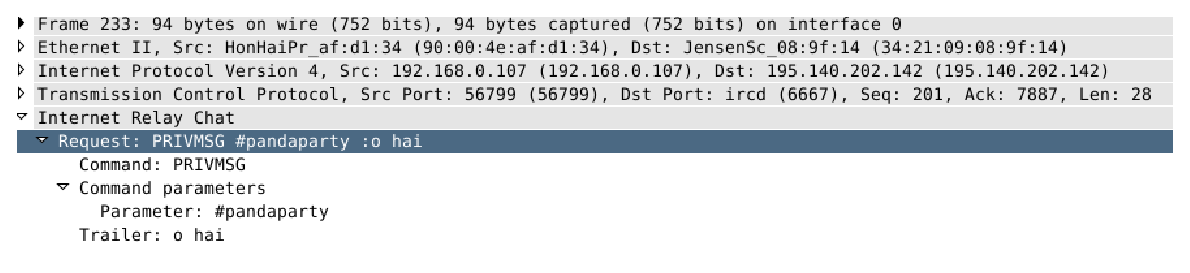
\includegraphics[width=6.9252in,height=1.4346in]{CryptographyandAnonymityformatted-img001.eps}
\end{center}
2 -- \textit{A TCP packet with SSL activated, containing the same data as the one depicted above}


\bigskip

3 -- \textit{A UDP packet in an OpenVPN UDP tunnel}

\begin{center}
\includegraphics[width=6.9252in,height=1.3362in]{CryptographyandAnonymityformatted-img002.eps}
\end{center}
4 -- \textit{An onion-layered packet sent through the TOR network}

\begin{center}
\includegraphics[width=6.9252in,height=1.3256in]{CryptographyandAnonymityformatted-img003.eps}
\end{center}

\bigskip


\begin{center}
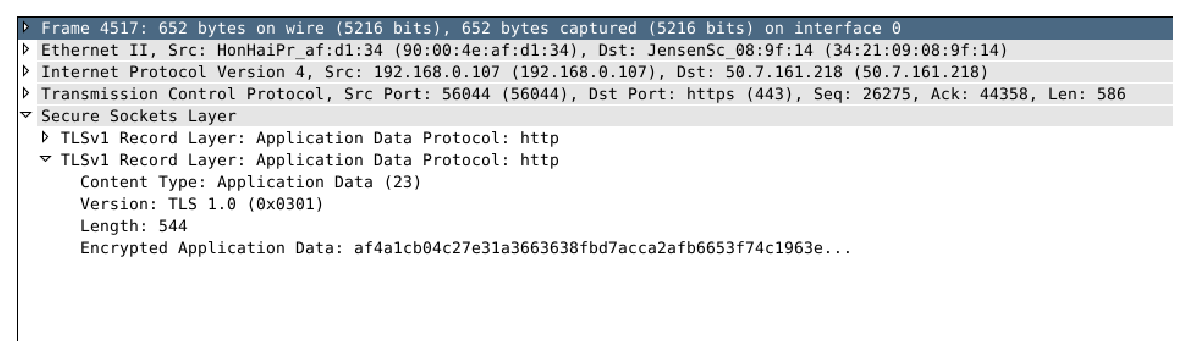
\includegraphics[width=6.9252in,height=1.9465in]{CryptographyandAnonymityformatted-img004.eps}
\end{center}
\end{document}
